\documentclass[showpacs,preprintnumbers,amsmath,amssymb,superscriptaddress,aip]{revtex4-1}
\usepackage{graphicx}
%\setlength{\parindent}{0in}

% General Latex  --------------------------------------------------
\def\beq{\begin{equation}}
\def\eeq{\end{equation}}
\def\beqar{\begin{eqnarray}}
\def\eeqar{\end{eqnarray}}
\def\nn{\nonumber}
\def\ol{\overline}
\def\para{\parallel}

% Operators  ------------------------------------------------------
\newcommand{\diff}[2]{\frac{d#1}{d#2}}
\newcommand{\diffs}[2]{\frac{d^2#1}{d#2^2}}
\newcommand{\pdiff}[2]{\frac{\partial#1}{\partial#2}}
\newcommand{\pdiffs}[2]{\frac{\partial^2#1}{\partial#2^2}}
\newcommand{\pdiffxy}[3]{\frac{\partial^2#1}{\partial#2 \partial#3}}
\newcommand{\pdt}{\partial_t}
\newcommand{\pdr}{\partial_r}
\newcommand{\pdth}{\partial_\theta}
\newcommand{\pdrr}{\partial^2_r}

\newcommand{\enum}[2]{{#1}\times10^{#2}} % 4.2x10^{3} = \enum{4.2}{3}

\newcommand{\vect}[1]{{\bf #1}}
%\newcommand{\vect}{\overrightarrow}
%\newcommand{\vect}{\vec}
\def\div{\nabla\cdot}
\def\grad{\nabla}
\def\curl{\nabla\times}
\newcommand{\gradpar}{\grad_\parallel}
\newcommand{\gradperp}{\grad_\perp}
\newcommand{\gradr}{\grad_r}
\newcommand{\defeq}{\ensuremath{\stackrel{\text{\tiny def}}{=}}}

\newcommand{\savg}[1]{\left<{#1}\right>}
\newcommand{\vavg}[1]{\left<{#1}\right>_V}
\newcommand{\thavg}[1]{\left<{#1}\right>_\theta}

% Variable names  -------------------------------------------------
\newcommand{\vpar} {v_\parallel}
\newcommand{\Apar} {A_\parallel}
\newcommand{\jpar} {j_\parallel}
\newcommand{\kpar} {k_\parallel}
\newcommand{\kperp} {k_\perp }
\newcommand{\vperp} {v_\perp }
\newcommand{\kthe}{k_\theta}

\newcommand{\Evec}{\ensuremath{\boldsymbol{{\rm E}}}}
\newcommand{\Bvec}{\ensuremath{\boldsymbol{{\rm B}}}}
\newcommand{\Jvec}{\ensuremath{\boldsymbol{{\rm J}}}}
\newcommand{\Fvec}{\ensuremath{\boldsymbol{{\rm F}}}}
\newcommand{\fvec}{\ensuremath{\boldsymbol{{\rm f}}}}
\newcommand{\vE}{\ensuremath{\boldsymbol{{\rm v}_{E}}}}
\newcommand{\bo}{\ensuremath{\boldsymbol{{\rm b}_0}}}
\newcommand{\bvec}{\ensuremath{\boldsymbol{{\rm b}}}}
\newcommand{\xvec}{\ensuremath{\boldsymbol{{\rm x}}}}
\newcommand{\yvec}{\ensuremath{\boldsymbol{{\rm y}}}}
\newcommand{\zvec}{\ensuremath{\boldsymbol{{\rm z}}}}
\newcommand{\vvec}{\ensuremath{\boldsymbol{{\rm v}}}}
\newcommand{\jvec}{\ensuremath{\boldsymbol{{\rm j}}}}

\newcommand{\bxgp}{\bvec\times\gradperp}

\newcommand{\vve}{\ensuremath{\boldsymbol{{\rm v}}_{e}}}
\newcommand{\vvi}{\ensuremath{\boldsymbol{{\rm v}}_{i}}}
\newcommand{\vpe}{v_{\parallel e}}
\newcommand{\vpi}{v_{\parallel i}}
\newcommand{\vvE}{\ensuremath{\boldsymbol{{\rm v}}_{E}}}
\newcommand{\vvD}{\ensuremath{\boldsymbol{{\rm v}}_{D}}}

\newcommand{\nuei}{\nu_{ei}}
\newcommand{\nuii}{\nu_{ii}}
\newcommand{\nue}{\nu_{e}}
\newcommand{\nuen}{\nu_{en}}
\newcommand{\nuin}{\nu_{in}}
\newcommand{\kpe}{\kappa_{\parallel e}}

\newcommand{\rs}{\rho_{s}}
\newcommand{\ri}{\rho_{i}}
\newcommand{\wci}{\Omega_{i}}
\newcommand{\wcix}{\Omega_{ix}}
\newcommand{\wce}{\Omega_{e}}
\newcommand{\tomega}{\tilde\omega}
\newcommand{\Isat}{I_{\rm sat}}
\newcommand{\fmie}{\frac{m_i}{m_e}}
\newcommand{\fmei}{\frac{m_e}{m_i}}


% Often used dimensions
\newcommand{\cm}{\rm cm}
\newcommand{\mm}{\rm mm}
\newcommand{\cmn}{{\rm cm}^{-3}}
\newcommand{\mn}{{\rm m}^{-3}}
\newcommand{\eV}{\rm eV}
\newcommand{\G}{\rm G}
\newcommand{\T}{\rm T}



\begin{document}

\title{A Linear Technique to Predict Non-Normal LAPD Turbulence}

\author{B. Friedman}
\email{friedman@physics.ucla.edu}

\author{T.A. Carter}

\affiliation{Department of Physics and Astronomy, University of California, Los Angeles, California 90095-1547, USA}



\begin{abstract}
In dynamical systems with highly nonorthogonal linear eigenvectors, non-modal linear analysis can be much more useful than normal-mode analysis in predicting turbulent properties. 
However, the non-trivial time evolution of non-modal structures makes quantitative prediction difficult. We present a technique using only linear calculations to overcome
this difficulty by modelling the effect that the advective nonlinearities have on spatial turbulent structures. Specifically, we model the nonlinearities as a periodic randomizing force with
period consistent with critical balance arguments. We apply this technique to a model of drift wave turbulence in the Large Plasma Device (LAPD) 
[W. Gekelman \emph{et al.}, Rev. Sci. Inst. {\bf 62}, 2875 (1991)], where non-modal effects dominate the turbulent system. 
We compare the resulting growth rate spectrum to that obtained from a nonlinear simulation, showing good quantitative agreement.
\end{abstract}

\maketitle

\section{Introduction}

Normal mode analysis -- the calculation of eigenvalues and eigenvectors of a linearized dynamical system -- has been used for the last two centuries to solve a number of problems ranging from
heat conduction along a solid bar to quantum mechanical energy states of atoms. Despite its wide-ranging success, normal mode analysis has seemingly failed in particular instances,
particularly in predicting the onset of turbulence in many hydrodynamic flows, where the turbulence is called subcritical. 
The reason for this failure was not clearly explained until the early 1990's when Trefethen and others attributed the pitfalls of normal mode analysis to the non-normality of linear operators of
dynamical systems~\cite{trefethen1993,trefethen2005} -- a non-normal operator or matrix is one that does not commute with its adjoint and consequently has 
eigenvectors that are nonorthogonal to one another. One consequence of eigenvector nonorthogonality is that even when all eigenvectors are stable and decay exponentially under linear evolution, 
superpositions of eigenvectors can grow, albeit transiently.
A paradigmatic illustration of this transient growth process for two nonorthogonal eigenvectors may be seen if Figure 2 of a review paper by Schmid~\cite{schmid2007}.
Physically, this means that certain types of fluctuations of the laminar state can access free energy from background gradients even though normal mode fluctuations cannot.
When combined with nonlinear effects, this allows for sustained subcritical turbulence.
Such behavior is obscured by traditional normal mode analysis, which only effectively describes the long time asymptotic behavior of fluctuations under the 
action of the linear operator. Transient growth events, which can dominate nonlinear turbulent evolution, require initial-value (non-modal) calculations rather than normal mode calculations.

Non-modal analysis has been embraced by the hydrodynamics community over the past two decades in the attempt to explain and predict subcritical turbulence. But the plasma community
still heavily relies on normal mode analysis to inform turbulent predictions and observations, with a few notable exceptions~\cite{camargo1998,camporeale2010,schekochihin2012}. 
Furthermore, non-modal treatments thus far have generally been explanatory rather than predictive and have centered around the transition to turbulence in subcritical systems rather 
than on properties of fully-developed turbulence.
This paper, in contrast, takes up the task of developing a quantitative approach to predicting turbulent properties using only non-modal linear calculations. 
The basic approach we take is to solve the linear initial value problem using an ensemble of random initial conditions, 
and then calculate the average growth rate of the solutions up to one nonlinear decorrelation time. We take this nonlinear decorrelation time to be a characteristic \emph{linear} time.
This procedure produces an effective growth rate spectrum that can be used to predict turbulent properties such as saturation levels.
While the concepts behind this technique are general enough to be applied to many nonlinear dynamical systems, the details will vary from system to system, 
so we restrict our treatment to one particular turbulence model.

The model is designed to describe a drift wave turbulence experiment conducted in the Large Plasma Device (LAPD)~\cite{gekelman1991}. LAPD is a linear machine with a straight magnetic $\mathbf{B}$ field.
Due to its large dimensions and high collisionality, LAPD is apt for fluid modelling. Thus, we use a reduced Braginskii~\cite{Braginskii1965} 2-fluid model:

\beqar
\label{ni_eq}
\pdt N = - {\mathbf v_E} \cdot \grad N_0 - N_0 \gradpar \vpe + \mu_N \gradperp^2 N + S_N + \{\phi,N\}, \\
\label{ve_eq}
\pdt \vpe = - \fmie \frac{T_{e0}}{N_0} \gradpar N - 1.71 \fmie \gradpar T_e  + \fmie \gradpar \phi - \nue \vpe + \{\phi,\vpe \}, \\
\label{rho_eq}
\pdt \varpi = - N_0 \gradpar \vpe  - \nuin \varpi + \mu_\phi \gradperp^2 \varpi + \{\phi,\varpi \}, \\
\label{te_eq}
\pdt T_e = - {\mathbf v_E} \cdot \grad T_{e0} - 1.71 \frac{2}{3} T_{e0} \gradpar \vpe + \frac{2}{3 N_0} \kpe \gradpar^2 T_e  \nonumber \\
- \frac{2 m_e}{m_i} \nue T_e  + \mu_T \gradperp^2 T_e +  S_T + \{\phi,T_e\},
\eeqar
where $N_0$ and $N$ are the equilibrium and fluctuating density, $\vpe$ is the fluctuating parallel electron velocity, $\varpi \equiv \gradperp \cdot (N_0 \gradperp \phi)$ is the potential vorticity
of the fluctuating potential $\phi$, and $T_{e0}$ and $T_e$ are the equilibrium and fluctuating electron temperature. The equations employ Bohm normalizations: lengths are
normalized to the ion sound gyroradius $\rho_s$, times to the ion cyclotron time $\omega_{ci}^{-1}$, velocities to the sound speed $c_s$, densities to the equilibrium peak density, and electron
temperatures and potentials to the equilibrium peak electron temperature. The profiles $N_0$ and $T_{e0}$ and other parameters are all taken from experimental measurements. $\phi_0$ 
does not appear in the equations because we model one particular experiment in which the equilibrium radial electric field was nulled by boundary biasing~\cite{schaffner2012}. 

The equations are global and partially linearized; the only nonlinearities retained are the advective nonlinearities in the Poisson brackets. 
We add artificial diffusion and viscosity terms with small numerical coefficients ($\mu_N, \mu_\phi, \mu_T = 10^{-3}$), 
used for numerical stability in nonlinear simulations, which are performed with the BOUT++ code~\cite{dudson2009}. We use periodic axial and zero value radial 
boundary conditions. Further details of the model, including validation studies, may be found in the references~\cite{Popovich2010a,Popovich2010b,Umansky2011,friedman2012b,friedman2013},
though we mention here that the model reproduces all statistical properties of the experimental turbulence within a factor of two, and in most cases, much better than that.

The nonlinear simulation reveals a fascinating property of the turbulence -- it is dominated by a nonlinear instability process despite being linearly unstable to drift waves
~\cite{friedman2012b,friedman2013}.
This nonlinear instability process, which was discovered by Drake et al.~\cite{drake1995} using a similar plasma model to ours, works as follows: 
long ($k_\para=0$) convective filaments transport density across the equilibrium density profile, setting up $k_\para=0$ density filaments (the same applies to the temperature). 
These filaments are unstable to drift waves causing a secondary drift wave instability to grow on the filaments. 
These drift waves, which have finite $k_\para$ and propagate primarily radially, nonlinearly couple to one another and reinforce the convective filaments.

Although the instability is called a nonlinear instability, the first part of the mechanism -- the transport of background density by the convective filaments -- is a linear one.
In fact, the other parts of the mechanism are driven by energetically conservative nonlinear interactions, 
meaning that the convective transport is the only step responsible for energy injection into the fluctuations from the laminar state.
Deriving an equation for the evolution of the energy from Eqs.~\ref{ni_eq}-\ref{te_eq}~\cite{friedman2012b,friedman2013}, we may symbolically write

\beq
\label{dEdt_def}
\diff{E(m,n,t)}{t} = Q(m,n,t) + D(m,n,t) + \sum_{m',n'} T(m,m',n,n',t).
\eeq
In this equation, $m$ and $n$ represent the azimuthal and axial Fourier mode numbers, respectively. 
Since Eqs.~\ref{ni_eq}-\ref{te_eq} are not explicitly dependent on $\theta$ and $z$, the energy equation is separable for every $m$ and $n$. 
Futher, $Q$ represents the linear energy exchange with the equilibrium (convective transport), $D$ the dissipation from irreversible processes
like collisions, and $T$ the nonlinear triad wave transfer. Since $\int f \{g,f\} dV = 0$, or equivalently $\sum_{m,m',n,n'} T(m,m',n,n',t)=0$, 
the Poisson bracketed advective nonlinearities in the model are energetically conservative and therefore do no inject or dissipate energy on the whole.
Consequently, the fluctuation energy originates completely from $Q$, the linear convective transport mechanism.

\begin{figure}
\centerline{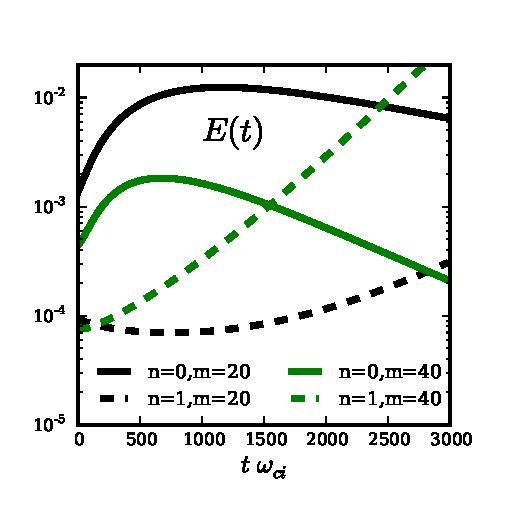
\includegraphics[]{transient_n0_n1_growth}}
\caption{The linear evolution of the energy of several Fourier modes starting from a turbulent initial state. The $n=0$ curves have an initial period of transient growth before exponentially decaying,
while the $n=1,m=20$ curve transiently decays before growing exponentially.}
\label{transient_n0_n1_growth}
\end{figure}

This convective transport of density filaments is akin to the paradigmatic ``lift-up'' mechanism in hydrodynamic shear flows whereby streamwise vortices drive streamwise streaks~\cite{krommes1999}.
Both are transient growth processes. We see this in our simulations by following the evolution of the energy of several Fourier $m,n$ modes after turning off the nonlinearities in an already
turbulent simulation. A few representative $m,n$ modes are shown in Fig.~\ref{transient_n0_n1_growth}. The transient growth of the filamentary structures is seen in the $n=0$ modes, 
which grow transiently before decaying exponentially at the rate of their least stable eigenmode. This kind of behavior is rather unituitive to some because all $n=0$ linear eigenmodes are stable, 
and the normal mode paradigm has conditioned us to believe that a linear superposition of such eigenmodes should decay. But as the hydrodynamics community discovered, linear
superpositions of nonorthogonal vectors may behave unintuitively.
Notice now that the $n=1,m=20$ mode decays transiently before growing exponentially with growth rate of the most unstable eigenmode at $n=1,m=20$. This isn't quite as interesting as the $n=0$
behavior, and it can occur in normal systems. Futhermore, it has no parallel in truly subcritical turbulence, but it can be helpful for interpreting later results.

We stress that Fig.~\ref{transient_n0_n1_growth} is obtained by \emph{linear} evolution from an initial turbulent state.
Since the transient growth, which is behind subcritical turbulence, is a purely linear phenomenon, it has long been a goal of researchers to predict the onset of subcritical turbulence using
only linear, non-modal calculations. It is our goal, however, to go a step further and use linear calculations to understand and even predict turbulent properties.
Such calculations would be much faster and easier to interpret than direct simulations of nonlinear equations. Perhaps one of the most useful statistical properties that we can use to describe
the turbulence -- and one that is conveniently ammenable to linear analysis -- is the turbulent growth rate spectrum.

\begin{figure}
\centerline{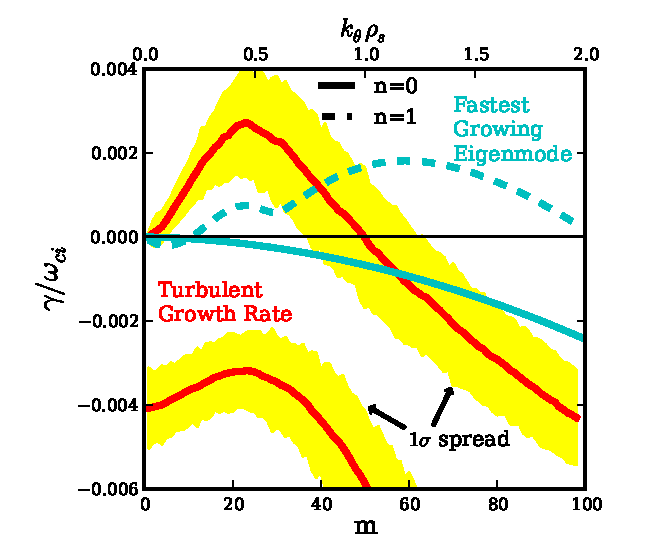
\includegraphics[]{spec_nl_gamma}}
\caption{The linear and turbulent growth rate $m$ spectra for $n=0$ (solid lines) and $n=1$ (dashed lines) Fourier components. The linear growth rates are those for the least stable eigenmodes at each
$n$ and $m$, while the turbulent growth rates represent $\pdiff{E}{t}|_{\rm{lin}}/2 E$ from the nonlinear simulation. The shaded region marks the $1 \sigma$ spread in the turbulent growth rate spectrum,
obtained from the distribution of growth rates calculated from the nonlinear simulation over a long time range.}
\label{spec_nl_gamma}
\end{figure}

To obtain the turbulent growth rate spectrum from the nonlinear simulation, we begin with the expression $\diff{E(m,n,t)}{t}\big|_{\rm{lin}} = Q(m,n,t) + D(m,n,t)$, 
which accounts for the total net energy injection at each $m,n$ into the fluctuations. 
An effective instantaneous growth rate $\gamma_{\rm{eff}}(m,n,t) = \diff{E(m,n,t)}{t}\big|_{\rm{lin}}/ 2 E(m,n,t)$ can then be defined. 
This effective growth rate is calculated from the spatial structure of the fluctuations, so it is well-defined for both turbulent fluctuations and eigenmode fluctuations. If calculated
from a linear simulation run for a sufficiently long time, $\gamma_{\rm{eff}}(m,n)$ is the same as the eigenmode growth rate of the least stable linear eigenmode for each $m,n$.
For turbulence, $\gamma_{\rm{eff}}(m,n)$ is generally not equal to an eigenmode growth rate, especially in the case where the system is non-normal.
We plot this growth rate in Fig.~\ref{spec_nl_gamma} for $n=0$ and $n=1$ components. The turbulent growth rate curves are calculated from this formula, 
averaged over a time of about $3 \times 10^{4} \ \omega_{ci}^{-1}$ during the saturated turbulent phase of the nonlinear simulation: $\gamma_{\rm{Turb}}(m,n) = \int \gamma_{\rm{eff}}(m,n,t) dt$. 
We show this turbulent growth rate along with the $1 \sigma$ contour, which indicates how greatly $\gamma_{\rm{eff}}(m,n,t)$ varies over time.
Along with these, the growth rates of the least stable (or most unstable) linear eigenmodes are shown.

As already stated, one sees from Fig.~\ref{spec_nl_gamma} that the linear eigenmodes are unstable for $n=1$ and stable for $n=0$ as expected for drift waves. 
However, the turbulent growth rates are positive for $n=0$ and low $m$ (which is subcritical-like), but negative for $n=1$ at all $m$. 
There was already a hint of this from the initial behavior of the curves in Fig.~\ref{transient_n0_n1_growth}, but this is a quantitative and more thorough picture.
Again, the $n=0$ energy injection is a manifestation of the convective filaments drawing energy from the equilibrium density gradient and depositing this energy into the density fluctuations.

Our goal now is to reproduce the turbulent growth rate curves in Fig.~\ref{spec_nl_gamma} without performing nonlinear simulations. This is difficult because the growth rates depend on turbulent
structures, which for non-normal systems, may be very different from eigenmode structures, and which change in time due to transient evolution.
It is clear, however, that the turbulent structures at any given time are a result of both linear evolution and nonlinear energy transfer. 
If we imagine that the nonlinearities randomize the turbulent structures at each wavenumber while the linearities evolve the structures
deterministically, we can develop a procedure for choosing proper spatial structures that may be used in calculating effective growth rates.

To elucidate this procedure, we begin by taking Eqs.~\ref{ni_eq}-\ref{te_eq} and Fourier decomposing in the azimuthal and axial directions.
Then, we discritize in the radial direction ($r \rightarrow r_0, r_1, \ldots, r_N $), and approximate radial derivatives with finite differences. 
The resulting system of equations may be written in matrix form:

\beq
\label{mat_eq}
\mathbf{B}_{m,n} \diff{\mathbf{v}_{m,n}(t)}{t} = \mathbf{C}_{m,n} \mathbf{v}_{m,n}(t) - \sum_{m',n'}  \mathbf{v}_{E,m-m',n-n'} \cdot \gradperp \left( \mathbf{B}_{m',n'} \mathbf{v}_{m',n'}(t) \right),
\eeq
where $\mathbf{v}_{m,n} = \left( N(r_0), N(r_1), \ldots, \vpe(r_0), \vpe(r_1), \ldots, \phi(r_0), \phi(r_1), \ldots, T_e(r_0), T_e(r_1), \ldots \right)_{m,n}^{T}$ is the state of the system,
and $\mathbf{B}_{m,n}$ and $\mathbf{C}_{m,n}$ are coefficient matrices that include the equilibrium information and finite difference coefficients. The first term on the RHS represents the linearities,
and the second term the nonlinearities.
The equations for different $m$ and $n$ are separated, although the nonlinearity couples the different $m$'s and $n$'s. 
In other words, eigenmodes with different $m$ and $n$ are orthogonal and linearly non-interacting. Note that for each $m,n$, there exist $4 \times N_r$ linearly
independent, but nonorthogonal eigenvectors. Hence forth, we drop the $m,n$ subscripts.

In order to use non-modal analysis to calculate growth rates and other measures, one must choose a norm and inner product with which to work. While any choice of
inner product is possible, including that which orthogonalizes all eigenvectors, a physically relevant one is generally preferred~\cite{camargo1998,schmid2007,camporeale2010}. The most commonly used
is an energy inner product. Recall that the inner product of two vectors may be written $\left< \mathbf{x},\mathbf{y} \right> = \mathbf{y}^{*} \mathbf{M} \mathbf{x}$,
where $^*$ stands for the conjugate transpose, and $\mathbf{M}$ is a positive-definite matrix. $\mathbf{M}$ should be chosen such that 
$||\mathbf{v}|| = \sqrt{\left< \mathbf{v},\mathbf{v} \right>} = \sqrt{E}$. That is, the norm of the state vector is the square root of the energy. Furthermore, it is often convenient in
computations to use the $L_2$-norm, $||\mathbf{u}||_2 = \sqrt{\sum_i |u_i|^2}$. These requirements can be accomplished through the change of variables $\mathbf{u} = \mathbf{M}^{\frac{1}{2}} \mathbf{v}$.
Then the linear portion of Eq.~\ref{mat_eq} becomes

\beq
\label{lin_eq_A}
\diff{\mathbf{u}}{t} = \mathbf{A} \mathbf{u},  \quad \rm{where} \ \mathbf{A} = \mathbf{M}^{\frac{1}{2}} \mathbf{B}^{-1} \mathbf{C} \mathbf{M}^{-\frac{1}{2}}.
\eeq
The eigenvalues of $\mathbf{A}$ are the same as those of $\mathbf{B}^{-1} \mathbf{C}$ because $\mathbf{M}^{\frac{1}{2}} \mathbf{B}^{-1} \mathbf{C} \mathbf{M}^{-\frac{1}{2}}$ is a similarity transformation.

The solution of Eq.~\ref{lin_eq_A} is

\beq
\label{lin_soln}
\mathbf{u}(t) = e^{\mathbf{A} t} \mathbf{u}(0).
\eeq
This solution depends on the initial condition $\mathbf{u}(0)$ in addition to the spectral properties of $\mathbf{A}$. For purposes of turbulent growth rate prediction, we are interested in
the behavior of $||\mathbf{u}(t)||$. Therefore, we introduce the growth ratio $G(t)$, which measures the amplification or reduction in the square root of the energy from an initial state:

\beq
\label{g_def}
G(t) = \frac{||\mathbf{u}(t)||}{||\mathbf{u}(0)||} = \frac{||e^{\mathbf{A} t} \mathbf{u}(0)||}{||\mathbf{u}(0)||}.
\eeq
It can be shown that this growth ratio is bounded from above by $G_{\rm{max}}(t) = ||e^{\mathbf{A} t}||$. Furthermore, $G_{\rm{max}}(t) = e^{\gamma_s t}$, where $\gamma_s$ is the spectral growth rate
(the real part of the eigenvalue with largest real part), if and only if $\mathbf{A}$ is normal~\cite{schmid2007}. Otherwise, $G_{\rm{max}}(t) > e^{\gamma_s t}$. 

It is common practice in normal mode analysis to look for the least stable eigenmode, the idea being that eventually the fastest growing structure will overcome the others.
For the non-modal case, it is common to study the properties of $G_{\rm{max}}(t)$, because if $G_{\rm{max}}(t) > 1$ at any time, there is a possibility of amplification, even if it is only transient.
This allows for the possibility of exciting subcritical turbulence, which is where non-modal analysis is most often applied. 
However, it can be misleading to study only $G_{\rm{max}}(t)$ when predicting specific properties of turbulence because
$G_{\rm{max}}(t)$ is only the upper envelope of all possible $G(t)$ curves. No one particular initial condition $\mathbf{u}(0)$ evolves along $G_{\rm{max}}(t)$. 
Furthermore, it isn't obvious what kind of spatial structure or structures will come to dominate a turbulent system. 
In non-normal systems, unlike in the normal systems, optimal structures don't amplify themselves, rather, they evolve while increasing the total fluctuating energy.

We illustrate $G_{\rm{max}}(t)$ along with $G(t)$ for several random initial conditions in Fig.~\ref{m20n0_time_evs} a), all at $n=0$ and $m=20$. Despite the fact that all eigenmodes at this
wavenumber are stable, there is the possibility for transient amplification by a factor of $20$. Further, a sample of randomly initialized vectors are all transiently amplified, but none display
optimal growth as compared to $G_{\rm{max}}(t)$. We show a zoomed-in view of these randomly initialized curves in Fig.~\ref{m20n0_time_evs} b).
It appears extremely unlikely to choose a random initial vector that either optimally amplifies the energy at any time or one that monotonically decays, which would be the case
if the initial vector were one of the linear eigenvectors. 

\begin{figure}
\centerline{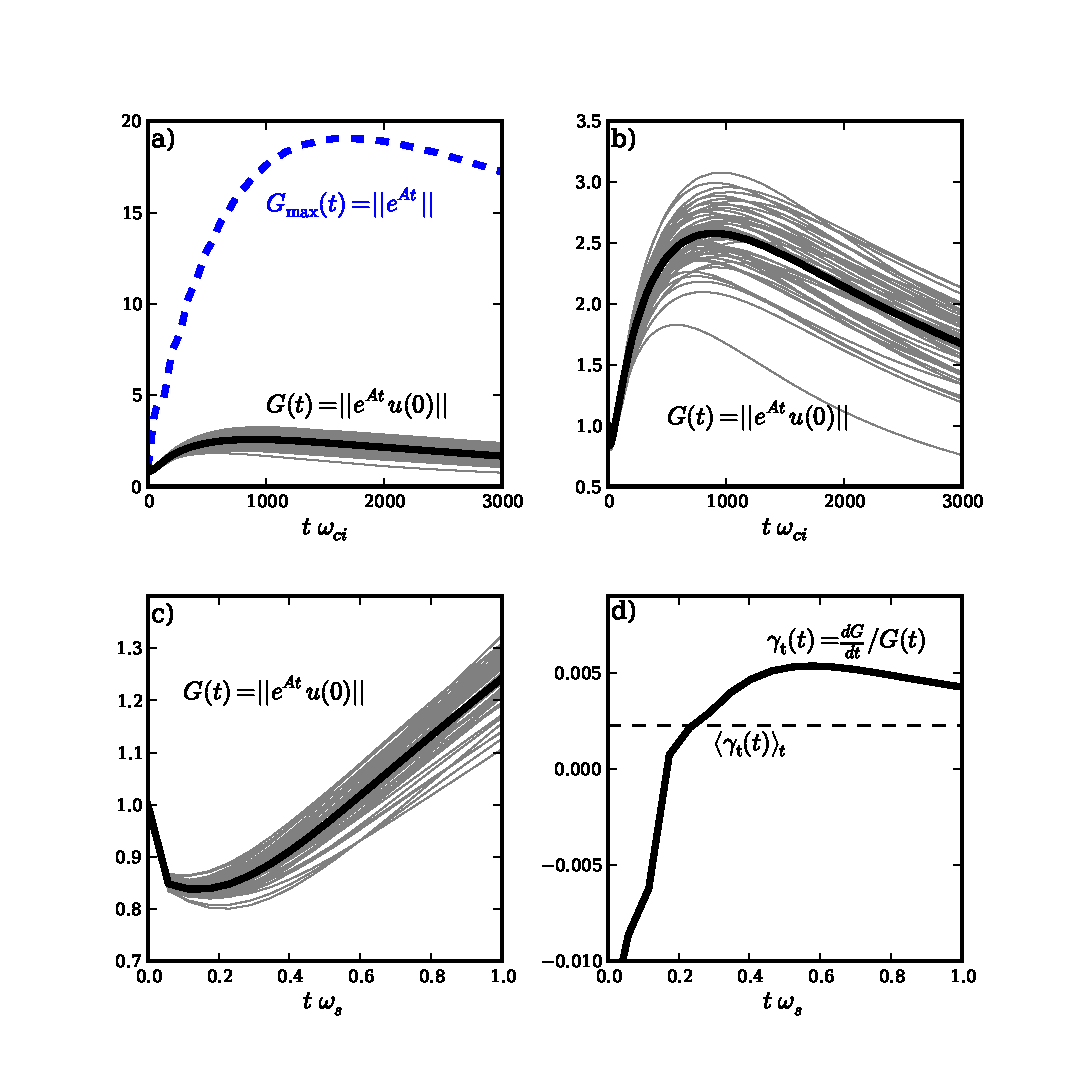
\includegraphics[]{m20n0_time_evs}}
\caption{a) The maximum growth ratio curve $G_{\rm{max}}(t)$ (dashed line) for $n=0,m=20$, and an ensemble of growth ratio curves (solid gray lines, with the solid black line the ensemble average)
that start with a random initial condition $u(0)$ and evolve under the linear operator. b) A zoomed in version of the ensemble of growth ratio curves. c) A further zoomed in version of the ensemble of
curves with a time range of $\omega_s^{-1}$, which is the characteristic linear time scale for drift waves. 
d) The instantaneous growth rate as a function of time of the the ensemble averaged growth ratio along with the average value over the time spanning $\omega_s^{-1}$.}
\label{m20n0_time_evs}
\end{figure}

Non-modal analysis has likely remained a qualitative endeavor due to the time-dependent growth properties of initial-value analysis as well as its intrinsic dependence on initial conditions.
The key to quantifying non-modal analysis and making it predictive is to successfully model the effect that the nonlinearities have on the transient linear processes. 
To this effect, we first note that the advective nonlinearity in Eq.~\ref{mat_eq} has the form of the state vector divided by a time $\tau_{\rm{nl}} \sim (v_E k_\perp)^{-1}$. This nonlinear
time scale is generally associated with the eddy turnover time or the time in which eddies become decorrelated. In light of this, we present a heuristical model of the nonlinearities 
as a randomizing force that acts on this characteristic nonlinear time scale.
Specifically, we start with a random initial condition, let it evolve linearly for a time $\tau_{\rm{nl}}$, and then re-randomized the system.
While the nonlinearities obviously do not affect the system in discrete time steps, this simplification provides a way to use linear non-modal analysis in a predictive manner.
In other words, there are certain spatial structures associated with the curves in Fig.~\ref{m20n0_time_evs} b) that change as a function of time. We consider only those structures from $t=0$, where
the structures are completely random, to $t = \tau_{\rm{nl}}$, and associate those structures with turbulent structures. These provide us with all we need to characterize the turbulence.

Now, since we do not know, \emph{a priori} at what level the turbulence will saturate, we cannot calculate the relative magnitude of $\tau_{\rm{nl}}$ from $(v_E k_\perp)^{-1}$ directly.
Thus, we invoke the conjecture of \emph{critical balance}, which posits that the nonlinear time scale equals the linear time scale at all spatial scales~\cite{schekochihin2012}. 
We can then estimate the nonlinear time scale as $\tau_{\rm{nl}} = \omega_{\rm{lin}}^{-1}$, the inverse of the linear frequency (at each $m,n$).
There are several choices of linear frequencies that we can use. Since we are dealing with a system of drift waves, $\omega_* = \frac{T_e m}{L_n r m_i \omega_{ci}^2}$ seems suitable, however,
$\omega_*$ is radially dependent, so it is not obvious which radius to choose. Alternatively, the linear frequency of the fastest growing eigenmode $\omega_s$ may be used. This is not a function
of radius, but $\omega_s = 0$ for $n=0$ eigenmodes, so one is forced to use $\omega_s$ for the fastest growing $n=1$ eigenmode at each $m$ to get a meaningful time scale. This is not wholly
unjustified, however, due to the inherent nonlinear coupling of different modes, which is evident in Eq.~\ref{mat_eq}.

To illustrate our procedure further, we show in Fig.~\ref{m20n0_time_evs} c) the randomly initialized linear evolution curves from start up until a time of $\omega_s^{-1}$. 
Then, in Fig.~\ref{m20n0_time_evs} d), we calculate the instantaneous growth rate as a function of time of the ensemble averaged curve over that time period.
The average of this instantaneous growth rate curve (the dashed line) gives the average ``Transient Growth Rate.''
In Fig.~\ref{spec_nl_transient_gamma}, we compare the Transient Growth Rate Spectra to the Turbulent Growth Rate Spectra, where we use $\omega_s^{-1}$ for $\tau_{\rm{nl}}$.
The $n=0$ curves in Fig.~\ref{spec_nl_transient_gamma} a) are fairly similar, especially when compared to the eigenmode spectra.
The $n=1$ curves, on the other hand, are not very similar, although they trend with $m$ in the same way, which is very different from the linear eigenmode trend.
The difference between the $n=1$ transient and turbulent growth rate spectra is due to nonlinear effects not captured by the simple transient calculation procedure. In particular, the turbulence
exhibits strong energy transfer from $n=0$ to $n=1$ Fourier components which is then dissipated by electron-ion collisions as the electrons stream along the field lines~\cite{friedman2012b}. 
This extra $n=1$ energy dissipation in the turbulent simulation is not a transient effect, and the $n=0$ to $n=1$ transfer is not a simple nonlinear mixing effect.

There is one more growth rate curve in Fig.~\ref{spec_nl_transient_gamma}, labelled ``Trans $\omega_s^{-1}$ cascade.'' We include this to address the apparent downshift (in $m$) of
the transient $\omega_s^{-1}$ curve in comparison to the turbulent curve. The downshift is a consequence of our oversimplification of the nonlinearity. Specifically, we
used $\omega_s^{-1}$ at each $m$ for the nonlinear time scale at that same $m$. As seen in Eq.~\ref{mat_eq}, $v_{m,n}$ is affected by every $\mathbf{v}_{E,m-m',n-n'} k^{'}_\perp$, not by only
$\mathbf{v}_{E,m,n} k_\perp$. Since we do not want to overcomplicate matters, we address this by posing a simple forward cascade model for the nonlinearity. That is, $v_{m,n}$ should be
most affected by the term with $m' = m/2 \rightarrow m-m' = m/2$, corresponding to eddy mitosis. Then, $\mathbf{v}_{E,m-m',n-n'} k^{'}_\perp \sim \mathbf{v}_{E,m/2} k^{'}_\perp/2 \sim \omega_{s,m/2}^{-1}$, 
so we use $\omega_s^{-1}$ at $m/2$ for the randomizing time scale at $m$ in deriving the ``Trans $\omega_s^{-1}$ cascade'' curves in Fig.~\ref{spec_nl_transient_gamma}. 
The $n=0$ curve matches well with the $n=0$ Turbulent Growth Rate curve at $m>20$, but poorly for $m<20$, which is expected because the cascade applies only at high $m$. \emph{A priori}, we
cannot determine the minimum $m$ for which the cascade should apply, so this method is simply explanatory.

\begin{figure}
\centerline{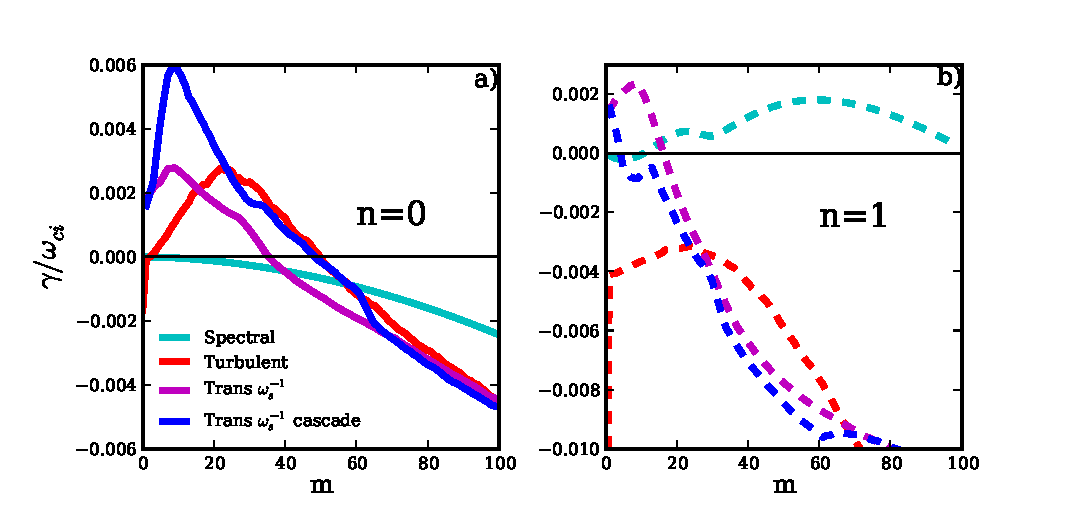
\includegraphics[]{spec_nl_transient_gamma}}
\caption{The linear, turbulent, and transient growth rate spectra. The transient growth rate spectra are calculated by the average growth rate over a time $\omega_s^{-1}(m,n=1)$ for the ensemble average
growth ratio curves with the cascade curve using $\omega_s^{-1}$ at $m/2$ rather than $m$.}
\label{spec_nl_transient_gamma}
\end{figure}

Nevertheless, our randomizing transient method, which requires only linear calculations, reproduces energetic growth properties of the turbulence that are not captured by eigenmode analysis.
Clearly, when the linear systems are highly non-normal, transient growth rate analyses should be performed in place of (or in addition to) linear eigenmode analyses. 
Furthermore, the transient growth rates should be used in the kinds of predictions that are currently made with eigenmode growth rates. 
For instance, quasilinear theory uses the most unstable eigenmode growth rate $\gamma_{s,max}$ to predict the turbulent saturation levels through the mixing length formula $\gamma/k_\perp^2$. 
Using this formula with $\gamma_{s,\rm{max}} = 0.002$ and $m=60$, one would predict a turbulent saturation level on the order of $0.1 \%$. 
On the other hand, using this formula with the transient values -- $\gamma_{t,\rm{max}} = 0.003, m=10$ -- we predict the saturation level on the order of $10 \%$,
which matches the saturation level in the nonlinear simulation.

In summary, non-modal linear calculations are more informative than normal mode calculations when the linear system under consideration is highly non-normal. In the specific case of a low-flow
LAPD experiment, a nonlinear instability with linear $k_\para=0$ drive dominates the energy dynamics of the turbulence. While this is a surprising result in light of normal mode analysis,
it is not at all surprising given the system's non-modal behavior. In general, non-modal initial-value analysis is difficult to quantify and make predictive, but using some simple nonlinear modelling,
we have shown that it is possible.

\begin{acknowledgments}

\end{acknowledgments}


%%%%%%%%%%%%%%%%%%%%%%%%%%%%%%%%%%%%%%%%%%%%%%%%%%%%%%%%%%%%%%%%%%%%%%%%%%%


\bibliography{refs}
%\bibliographystyle{unsrt}


\end{document}
